\documentclass{article}
\usepackage[T1]{fontenc}
\usepackage{lmodern}
\usepackage{graphicx}
\usepackage{amsmath,amssymb}
\usepackage[a4paper,margin=2cm]{geometry}
\usepackage[absolute,overlay]{textpos}
\setlength{\TPHorizModule}{1mm}
\setlength{\TPVertModule}{1mm}
\usepackage[indonesian]{babel}
\usepackage{hyperref}
\setlength{\emergencystretch}{2em}
% unit: Halaman 23

\begin{document}

% === Halaman 23 (llm) ===

\vspace{264.33mm}

Input: $\text{101010}$
Baris = $\text{10} = 2$
Kolom = $\text{0101} = 5$
Luaran = $13 = 1101$

\vspace{50mm}

\begin{itemize}
    \item Setiap baris di dalam S-box adalah permutasi angka-angka $0, 1, 2, \dots, 15$.
    \item Mengubah satu bit di dalam input S-box mengakibatkan perubahan paling sedikit 2 bit pada output S-box
\end{itemize}

$\rightarrow$ prinsip \textit{confussion}

% deskripsi: Empat tabel S-box ($S_5, S_6, S_7, S_8$) yang digunakan dalam proses substitusi kriptografi, dengan tabel $S_5$ menunjukkan proses indexing baris dan kolom.
% bbox normalisasi: [0.2100, 0.0000, 0.9200, 0.8900]
\begin{textblock*}{149.10mm}(44.10mm,0.00mm)
\noindent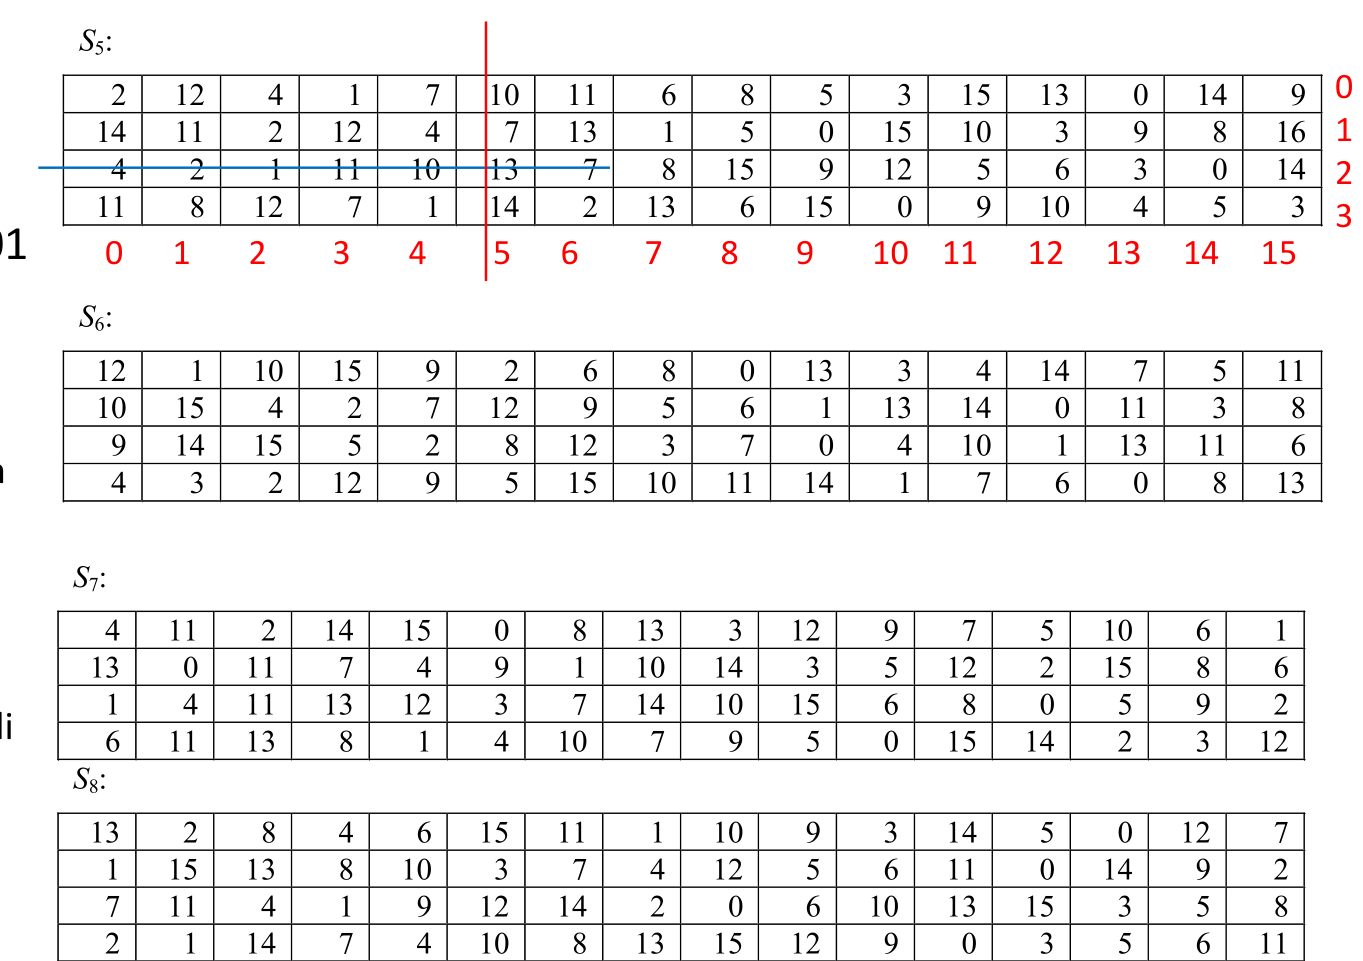
\includegraphics[width=149.10mm,height=264.33mm]{../../images/llm/page_023_img_01.png}%
\end{textblock*}

\end{document}
